\documentclass[a4paper,11pt]{article}
\usepackage{graphicx} % Required for inserting images
\usepackage{lipsum}
\usepackage{biblatex}
\usepackage{amsmath}
\usepackage{amsfonts}
\usepackage{amsthm}

\newtheorem{theorem}{Theorem}
\newtheorem*{problem}{Problem}
\theoremstyle{definition}
\newtheorem{definition}{Definition}
\addbibresource{bibmain.bib}
\title{Partial Optimal Transport}
\author{Romain Gambardella}
\date{January 2025}

\begin{document}

\maketitle

\section{Abstract}

In his paper \textit{The Optimal partial transport problem} (\cite{fig}), Alessio Figalli studies the transportation of a specific amount of mass beetween two densities f and g, minimizing a transportation cost, typically $c(x,y) = |x-y|^2$ in $\mathbb{R}^n$. This is a generalisation of classical optimal transport, where one is interested to transport all the mass from f to g.

This generalization permits to study unbalanced cases where f and g do not have the same amount of mass. Moreover, this problem has practical implications, notably in \cite{SPOT} the authors use it to implement a shape matching algorithm that is robust to outliers.

In this paper, Alessio Figalli uses the function $C(m)$ which is the minimal cost associated to transporting m units of mass, and uses it's convexity properties to prove the unicity of the solution. 

The paper presents the first proof of existence and unicity of the solution in the general case, and gives an in-depth study of the regularity of the transport map. It extends a result of Caffarelli and McCann who studied the problem only for distributions with disjoint support.
\section{Introduction}:

The problem of partial optimal transport was first introduced and studied by Caffarelli and McCann in \cite{caff}. 
It is a direct extension of the problems of Monge \cite{monge} and Kantorovich \cite{Kant} that we have seen in class. In these works one is concerned to assign the production of mines in the countrysides to facilities to process ore, minimizing the transportation cost induced by the transportation of materials. The local production and processing capacity are modelled by distributions $f$ and $g$ on the ambiant space ( in this example $\mathbb R^2$ ) and the total capacity of production is assumed to be the same as the total capacity of the factories, in other words $\int f = \int g$. \\

Most of the subsequent work on this problem kept this assumption; in particular the celebrated theorem of Brenier \cite{Brenier} needs balanced distributions to apply. 

However, even on the basic example one can see that there is no reason for the mines and the factories capacity to be equal ; in reality one could hope to have spare factories to cope with emergency. In multiple situations the partial optimal transport thus appear, which can be formulated as follow : given a distribution of local production capacity and local processing capacity, compute the best plan to generate an amount $m$ of processed ore at the best possible cost. \\

\subsection{Formalization of the problem}
The paper studies the optimal partial transport problem, which can be formalized ( in a Kantorovitch \cite{Kant} way ) in the following paragraphs. \\

Let f,g be two densities in $L^1(\mathbb{R}^d)$, and let $\Gamma^{\leq f,\leq g}$ denote the set of nonegative finite Borel measures on $R^d \times R^n$ whose marginals are respectively dominated by f and g : \\

$\gamma (A \times \mathbb{R}^n) \leq \int_A{f(x)dx} $ and 
$\gamma (\mathbb{R}^n \times A) \leq \int_A{g(x)dx} $ for all $A \in \mathcal{B}(\mathbb{R}^n)$ \\

The mass transported by $\gamma$ is defined as : $m(\gamma) = \gamma(\mathbb R^n \times \mathbb R^n )$. We denote the set of nonnegative finite Borel measures whose marginals are respectively dominated by f and g and whose mass is greater or equal to $m$ by $\Gamma^{\leq f,\leq g}_m$.

Given a cost function $c:\mathbb R^n \times\mathbb R^n \rightarrow {\mathbb R}$, the cost associated to $\gamma$ is defined as : $C(\gamma) = \int{c(x,y)d\gamma(x,y)}$.
\begin{definition}
Let $m_{max}$ denote $\max(\int f, \int g)$ the maximum mass that can be transported. We define, for $m<m_{max}$ the cost of transporting m units of mass as : 

\begin{align*}
     C :  \mathbb R_+ &\to   \overline{\mathbb R}_+ \\
      m  &\mapsto  \inf \{ C(\gamma),\gamma \in \Gamma^{\leq f,\leq g}_m \}
\end{align*}
where we use the convention that $\inf (\emptyset) = +\infty$
\end{definition}
Moreover, let $\Gamma^0(m)$ be the set of mesures of $\Gamma^{\leq f,\leq g}_m$ that are optimal for a certain mass $m$.

There are several questions that need to be answered : 
\begin{itemize}
    \item existence of the optimal map : is this set $\Gamma^0(m)$ non empty  ? 
    \item unicity of the solution : if an optimal map for a mass $m$ exists, is it unique ? We will, as in Figalli's paper, mostly focus on this question.
\end{itemize}

First let us see that the unicity property is non-trivial in this case. Let $m_{min} = \int{f(x)\wedge g(x) dx}$ be the mass common to f and g. Then for any density $h \in \mathbb L^1(\mathbb R^n)$ such that $h$ is dominated by $f \wedge g$, we have that $\gamma = (Id\times Id)_\# (h)$ is a valid coupling of cost $0$. So, for $m \leq m_{min}$, we get $C(m) = 0$ and for $m < m_{min}$, there are multiple partial maps that are optimal and the set of optimal partal maps can be trivially described by $$\forall m < m_{min} ,
 \Gamma^0(m) = \{(Id\times Id)_\# (h),  \int h = m, h\leq f\wedge g\}$$


The difficulty arises when trying to understand what happens when $m_{min} < m \leq m_{max}$, which is the focus of Figalli's paper. \\



\subsection{Contributions}

In \cite{caff}, Caffarelli and McCann already studied the properties of the partial transport plan. 

However, their work show the unicity only when f and g have disjoint support, using Kantorovitch duality and a tariff-free point at infinity. \\

The paper of Figalli get rid of the above limitation and takes a very different approach.

More precisly, Figalli proves the unicity for all density in $\mathbb{L}^1(\mathbb R^n)$ compatly supported and all mass $m \in [m_{min},m_{max}]$, for the cost $c(x,y) = |x-y|^2$. To prove the unicity of the solution, Figalli's show that the transport map associated to a mass m is unique whenever $C(m)$ is locally strictly convex at $m$, and then he proceeds to show the strict convexity of C(m). He does not use duality results. Instead, he makes heavy use of Brenier's theorem.

Moreover, Figalli's proves important properties such as the monotonicity of the active regions as $m$ increases, in the general case.

\subsection{Plan of the project}
To begin with, in \ref{sec:numerics}, I give a way to compute discrete maps with a proof inspired from Figalli's continuous case.

In the rest of the project I use this method to do several numerical experiments to illustrate Figalli's theorem, in the discrete case ( even if Figalli's paper is focused on the continuous case, the discrete case gives a good intuition of what is going on ).

In \ref{ref:propertiesC} I proceed by giving simple proofs of properties of the transportation cost function C that are proved in Figalli's paper.\\ 

Then, I proceed to extend the unicity proof given in Figalli's paper to the discrete case, in the case where the cost fonction $c(x,y)$ is injective. Moreover, I simplify the proof of the continuous case where $c(x,y) = |x-y|^p$, so as not to use Brenier theorem ( Figalli uses it extensively ).\\

%Finally, I illustrate some of Figalli's theorems such as the monotonicity theorem, stated without proof, in the discrete case.


\subsection{Notations}
In this report : 
Given two densities f and g, $f \wedge g$ and $f \lor g$ denote the pointwise minimum of f and g.

For simplicity, we sometimes refer by C(m) the function $m \mapsto C(m)$.

TODO : define $\gamma_0 \lor \gamma_1$ the min of two measures.
\section{Main body}

\subsection{Computing a partial transport map}\label{sec:numerics}

To compute the optimal transport plan, we follow the methodology of Caffarelli and McCann \cite{caff} and we add Dirac mass isolated at infinity as a tariff-free reserve. \\

More precisely, we construct a new optimal transport problem from the partial problem. The solution of this optimal transport problem gives then a way to get the solution of the partial problem. 

We start from a partial optimal transport problem : $\inf \{C(\gamma),\gamma \in \Gamma^{\leq f,\leq g}_m \}$,  with $f$ and $g$ in some space $E$, some positive cost c, and $m<m_{max}=\max(\int f, \int g)$.


We extend $E$ by adding a new point which gives a new space $\hat E=E \cup \hat \infty$. Then we create a new cost $\hat c(x,y)$ defined on $\hat E$ by : 

$$\hat c(x,y) = \begin{cases}
c(x,y) & \text{if } x \in E, y\in E \\
0 & \text{otherwise}
\end{cases}
$$

Then the two distributions are balanced : $\int \hat f =\int \hat g = \int f + \int g -m$. The new problem to be solved is then : 
\begin{equation}
\tag{$\hat P$}
\begin{aligned}
    \label{prob:Pprime}
    &\text{Minimize }  \hat C(\hat \gamma) = \int_{\hat E \times \hat E} \hat c(x,y) d\hat \gamma \\
    &\text{over all } \hat \gamma \text{ such that the first and second marginals of } \hat \gamma \text{ are } \hat f \text{ and  } \hat g.
\end{aligned}
\end{equation}

Then we let $\hat f$ and $\hat g$ be new densities on $\hat{E}$ equal to $f$ and $g$ on $E$ and with mass at infinity $\hat g(\hat \infty) = \max(0,\int f-m)$ and $\hat f(\hat \infty) = \max(0,\int g-m)$.

\begin{theorem}
    If $\hat \gamma \in \Gamma^{\leq \hat f,\leq \hat g}$ is a solution to the problem \ref{prob:Pprime} defined above, then $\hat \gamma$ restricted to $E \times E$ gives a solution to the partial problem. \\
    Conversely, for every solution $\gamma_m$ of the partial problem, there exists a solution $\hat \gamma$ to the problem \ref{prob:Pprime} such that $\hat \gamma$ restricted to $E \times E$ gives a solution to the partial problem.
\end{theorem}

\begin{proof}
For the proof, we draw inpiration from the paper of Figalli \cite{fig}.

Let $\hat \mu \in \Gamma^{\leq \hat f,\leq \hat g}$ be a solution to the problem \ref{prob:Pprime}.
Then using the constraints on the marginals of $\hat \mu$ we get that \begin{itemize}
    \item $\hat \mu(E \times \hat E) = \int f$
    \item $\hat \mu(E \times \{\hat \infty\}) \leq \hat \mu(\hat E \times \{\hat \infty\}) = \int f - m$
\end{itemize} 

As $\hat \mu(E \times \hat E) = \hat \mu(E \times E)+\hat \mu(E \times \{\hat \infty\})$, we get that $\hat \mu(E\times E) \geq m$.

Let us denote by $\mu$ the restriction of $\hat \mu$ to $E\times E$. Then $\mu$ has mass greater than m, and its marginals are equal to f and g. Thus, $\mu$ is in $\Gamma_m^{\leq f, \leq g}$. Moreover, we have that $\hat C (\hat \mu) = C(\mu)$
Now we need to prove that $\mu$ is optimal, that is, that $C(\mu) \geq C(\nu) $ for all $\nu$ in $\Gamma^{\leq f, \leq g} _m$.\\

Let $\nu \in \Gamma^{\leq f, \leq g}_m$, and let $\nu_0, \nu_1$ be it's first and second marginals respectively. Let $\gamma_0$ and $\gamma_1$ denote respectively the measures of density f and g on E. Let $\hat \nu$ be the nonnegative Borel measure on $\hat E \times \hat E$ defined as : $\hat \nu = \nu + (\gamma_0-\nu_0)\otimes \delta_{\hat \infty}+ \delta_{\hat \infty}\otimes (\gamma_1-\nu_1) + (m(\gamma) - m). \delta_{\hat \infty} \otimes \delta_{\hat \infty}$.

Then : \begin{itemize}
    \item $\nu$ is a valid nonnegative Borel measure as a sum of nonnegative Borel measures.
    \item the marginals of $\hat \nu$ have respectively density $\hat f$ and $\hat g$.
    \item the cost $ \hat C(\hat \nu)$ is equal to $C(\nu)$.
\end{itemize}

So, $C(\nu) = \hat C(\hat \nu) \geq  \hat C(\hat \mu) = C(\mu)$ ( because $\hat \mu$ minimizes \ref{prob:Pprime} ). $C(\mu) \geq C(\nu) $ for all $\nu$ in $\Gamma^{\leq f, \leq g} _m$, so $\mu$ is a solution of the partial problem.

Conversely, if $\nu$ is a solution to the partial problem, then  $C(\nu) = \hat C(\hat \nu) =  \hat C(\hat \mu) = C(\mu)$, so $\hat \nu$ is a solution to \ref{prob:Pprime}. 

\end{proof}

The proof of this theorem gives us a way to find a partial map. It suffices to solve the optimal transport problem \ref{prob:Pprime} on $E\cup{\hat \infty}$, and then to restrict this solution to $E$ to get a solution of the partial transport problem. In the figures \ref{fig:coupling} \ref{fig:partialmap} are plotted the partial map that \\

\begin{figure}
        \centering
        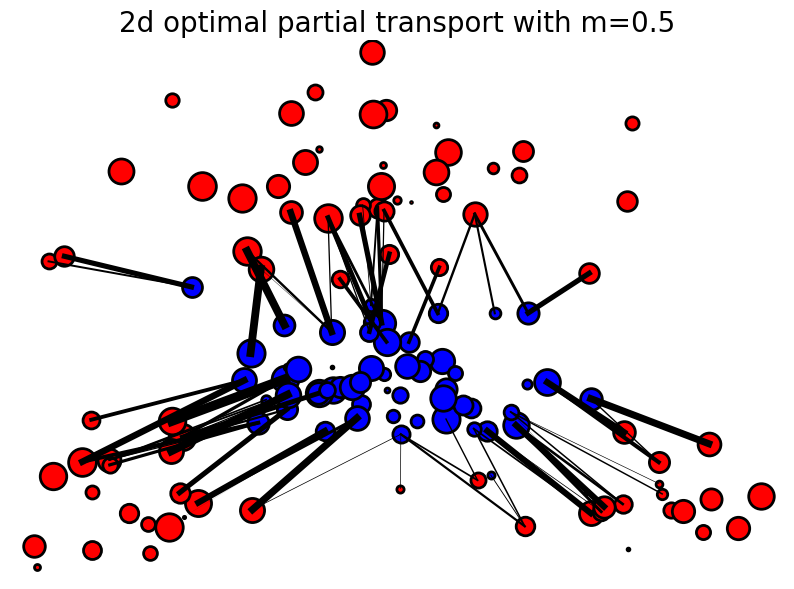
\includegraphics[width=0.8\linewidth]{image/partialmap2}
        \caption{Partial map beetween two densities computed using two points at infinity}
        \label{fig:partialmap}
    \end{figure}
    \begin{figure}
        \centering
        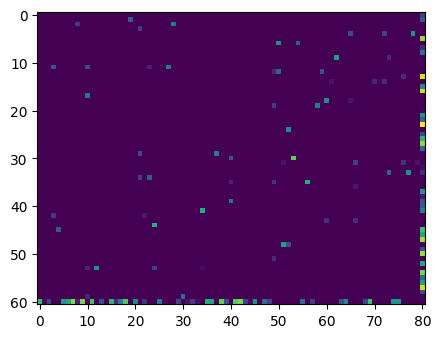
\includegraphics[width=0.8\linewidth]{image/Optimal coupling of mass 0.5 computed using two points at infinity.png}
        \caption{Optimal coupling of mass 0.5 computed using two points at infinity}
        \label{fig:coupling}
    \end{figure}

\newpage

\subsection{Properties of C(m)} \label{ref:propertiesC}
First, let us prove a few simple properties of the cost function.
\begin{theorem}[Convexity of C(m)]
    \begin{align*}
     C :  \mathbb R_+ &\to   \overline{\mathbb R}_+ \\
      m  &\mapsto  \inf \{ C(\gamma),\gamma \in \Gamma^{\leq f,\leq g}_m \}
\end{align*} is nondecreasing and convex on $[0,m_{max}]$, and equal to 0 on $[0,m_{min}]$, where $m_{min} = \int f\land g$ and $m_{max} = \min(\int f,\int g)$.
\end{theorem}

\begin{proof}
    We have already proven in the introduction that when $m \leq m_{min}$, we get that $C(m) = 0$.  \\

    The nondecreasing property is induced by the inclusion $\Gamma^{\leq f, \leq g}_{m_2} \subset \Gamma^{\leq f, \leq g}_{m_1}$ for any $m_1 \leq m_2$.\\
    
    The convexity property is proved in \cite{fig} using the existence of a minimizer; here, we slightly change the proof so as to not use this assumption.\\
    
    Let $0\leq m_1 \leq m_2 \leq m_{max}$.
    Let now $\epsilon>0$, and let $\gamma_1 \in \Gamma^{\leq f, \leq g}_{m_1},\gamma_2 \in \Gamma^{\leq f, \leq g}_{m_2}$ be two couplings such that : $\begin{cases}
        m(\gamma_1) \geq m_1, m(\gamma_2) \geq m_2 \\
        C(\gamma_1) \leq C(m_1)+\epsilon, C(\gamma_2) \leq C(m_2)+\epsilon
    \end{cases}$\\
    
    
    Then for any $\alpha \in [0,1]$ : 
    $$C(\alpha \gamma_1 +(1-\alpha)\gamma_2) = \alpha C(\gamma_1)+ (1-\alpha)C(\gamma_2) \leq \alpha C(m_1)+ (1-\alpha)C(m_2)+\epsilon$$
    As $m(\alpha \gamma_1 +(1-\alpha)\gamma_2) = \alpha m(\gamma_1) +(1-\alpha)m(\gamma_2) \geq \alpha m_1 +(1-\alpha)m_2$, we get that $C(\alpha m_1 +(1-\alpha)m_2) \geq \alpha C(m_1)+ (1-\alpha)C(m_2) + \epsilon$.

    As this property is true for all $\epsilon>0$, $m \mapsto C(m)$ is convex on $[0,m_{max}]$.
\end{proof}

An illustration of this theorem in the discrete case of \ref{fig:coupling} is given in Figure \ref{fig:conv};

\begin{figure}
    \centering
    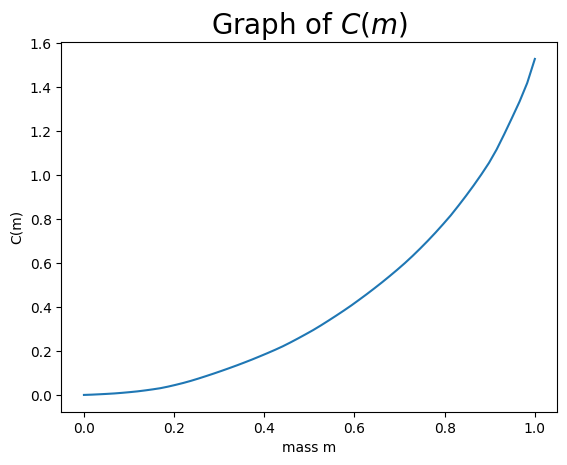
\includegraphics[width=0.8\linewidth]{image/convexity.png}
    \caption{Illustration of the convexity property of the transport cost function}
    \label{fig:conv}
\end{figure}

For now on, we assume the existence of an optimal transport map. Figalli in his paper briefly mentions that a minimizer always exists for $m\leq m_{max}$
Now, we follow Figalli who proceeds to prove the following theorem : 

\begin{theorem}[Strict convexity implies unicity]
    Let $m_{min} < m \leq m_{max}$. If the set of minimizers $\Gamma^0(m)$ is not empty, and if $m \mapsto C(m)$ is strongly convex in m, $\Gamma^0(m)$ is a singleton.
\end{theorem}

\begin{proof}
Let $m>0$. Suppose there are two distinct couplings $\gamma_0, \gamma_1 \in \Gamma^{\leq f, \leq g}_m$ such that $C(\gamma_0) = C(m), C(\gamma_1) = C(m)$. Then $\gamma_0 \lor \gamma_1$

Then 
\end{proof}


\subsection{unicity property}

prove in the discrete case

illustrate

\subsection{monotonicity}

illustrate









Presentation of the method(s).
Theoretical guarantees.
Numerics.
\section{Conclusion and perspective (~1 page)}
Summary of the result obtained: pros and cons (limitation, problems, errors in the articles, etc)
Possible improvement/extension
\section{Connexion with the course.}
What are the notions/results/algorithms presented in the course that are used or related to the one presented in this paper?


\printbibliography
\end{document}
